\section{Discussion}

The goal of this paper is to accurately classify light curves as representing potential exoplanets amongst many false positive cases. The binary model focused on the most common false positive occurring from eclipsing binary systems. The multiclass model attempts to include a separation between deep eclipsing binaries and shallow eclipsing binaries. Further cases can be added to give more possible classifications but for now the most important categories were covered.

The results found in this work demonstrate that 1D CNNs can distinguish confirmed transiting systems from eclipsing binaries with high performance. Unlike other papers, these results come from minimally processed Kepler light curves and show time can be saved on processing the data. However, there was still some classification difficulty as the eclipsing binary population produced non uniform errors, with shallow depth eclipsing binaries representing the principal source of confusion. 

\textbf{(Should I add a comparison to other papers which used higher preprocessing?)}

The data preparation did not apply any sigma-clipping of the normalized light curves. This was due to previous experiments showing that any application of clipping reduced the binary model across all metrics. The final decision to remove clipping, was motivated by the concern of outlier rejection accidentally removing important astrophysical information. Table~\ref{tab:clipping_comparison} shows the difference in the binary model metrics when applying sigma clipping to when it was not used.

\begin{table}[h]
    \centering
    \begin{tabular}{lccc}
        \hline
        \textbf{Metric} & \textbf{Sigma Clipping} & \textbf{No Clipping} & \textbf{Improvement} \\
        \hline
        Accuracy  & 83.28\% & 93.17\% & +9.89 pp \\
        Precision & 79.18\% & 89.46\% & +10.28 pp \\
        Recall    & 91.64\% & 98.50\% & +6.87 pp \\
        F1 Score  & 84.95\% & 93.76\% & +8.81 pp \\
        ROC-AUC   & 0.881   & 0.978   & +0.097 \\
        \hline
    \end{tabular}
    \caption{Comparison of binary CNN performance with and without sigma clipping during light-curve preprocessing. The improvement represents the absolute percentage-point change after removing sigma clipping, with ROC-AUC reported as an absolute change. Due to the improvements, sigma clipping was therefore excluded from all models.}
    \label{tab:clipping_comparison}
\end{table}

The binary model produced strong results which indicate it is very efficient in classifying distinctions between real and fake transit cases. Table~\ref{tab:metrics_table} shows the favourable results from the binary model test. An accuracy of 93\% indicates the model does not overall struggle handling the data. The precision and recall of 88\% and 98\% respectively show there is little to no issue classifying true transits appropriately. The recall shows the model found almost all of the transits which were used in the test. The precision however represents the reliability that a transit classification is truly a transit. While it is high, there is still 12\% of transit classifications which were actually eclipsing binaries.

While some light curve instances contained unusual features which may affect classification, there are also cases which manage to trick the binary classifier. Figure~\ref{fig:good_vs_bad_examples} shows a collection of correctly and incorrectly classified example instances used in testing. For the correctly classified cases, the top left plot shows a true transit instance. It appears visually similar to the top right plot, which depicts a false positive eclipsing binary. This demonstrates the difficulty of working with the intricate light curve data, as visually similar standardized inputs can result from different classes.

As for the eclipsing binaries, the bottom left shows an instance which was correctly classified. The alternating eclipse depths provide a clear feature expected from an eclipsing-binary system. The bottom right plot is a transit incorrectly classified as an eclipsing binary. Repeated downward features with varying standardized depths can be observed in the data, which may have contributed to the model incorrectly identifying the instance as an eclipsing binary. The exact source of these features cannot be determined from the light curve alone and could result from astrophysical variability, instrumental effects, or the processing of the observations.

\begin{figure}
    \centering
    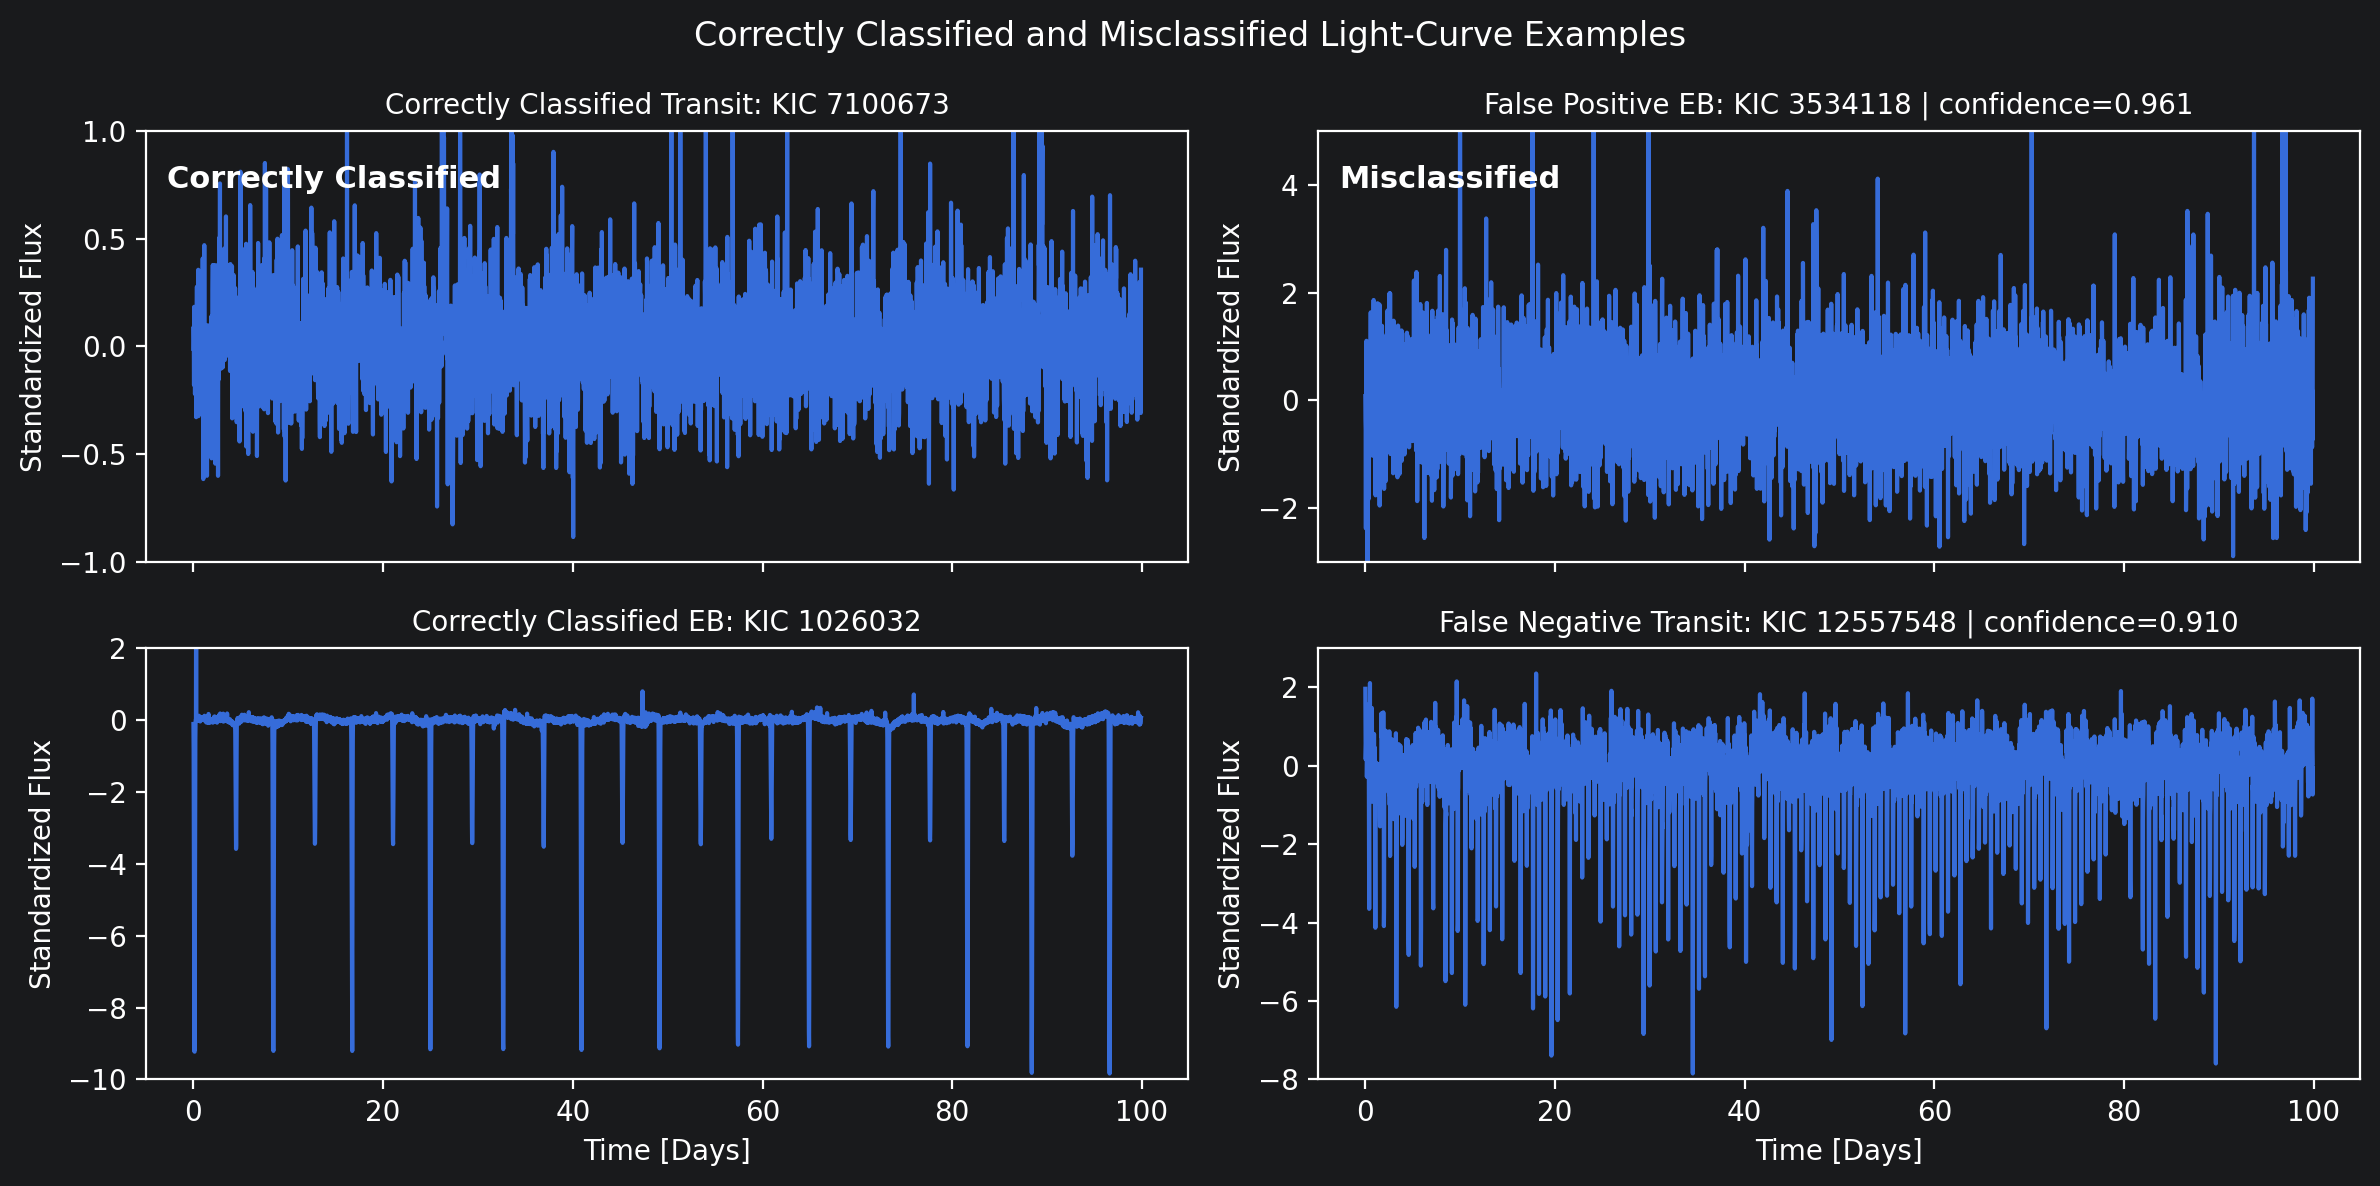
\includegraphics[width=0.9\linewidth]{figures/images/good_bad_binary_examples_2x2.png}
    \caption{Examples of correctly classified and misclassified light curves from the binary CNN. The left column shows correctly classified instances of a transit and eclipsing binary 100-day chunk. The right column shows an instance of both a transit and eclipsing binary which was misclassified by the binary model. The light curves shown are from after standardization and represents exactly the data provided to the model for training and testing. Limits on the plotted y-axis were applied to focus on the main density of data exclusing outliers.}
    \label{fig:good_vs_bad_examples}
\end{figure}

It can be seen from the confidence histogram that a large number of misclassified instances were found in the high-confidence ranges. One likely factor is the depth of the transits or eclipses, which can first be seen in the box plot in Figure~\ref{fig:depth_boxplot_fp}, where the high-confidence group has the most consistent collection of low-depth cases. This is further supported by the high-confidence false positives, where over 80\% of the unique systems were matched to shallow eclipsing binaries. This suggests that the shallow EB class is important to separate from the transit and deep EB cases, as these systems can be confidently mistaken for exoplanet-like transits.

The final decision for a split between shallow and deep eclipsing binary cases was needed for creating the multiclass model and Figure~\ref{fig:mc_threshold_find} gave the best representation for determining the threshold. The histogram shows how majority of misclassified eclipsing binaries come from relative eclipse depths of 0.01 or less. Totalling up the ratios, 42.1\% (160/380) of eclipsing binaries with depths less than 0.01 were misclassified while only $\sim1.0\%$ (11/1073) of those with depths greater than 0.01 being misclassified. The substantial difference in confusion rate provides good justification for the 0.01 operational depth split boundary.

Compared to the binary CNN model, the multiclass model performed a little poorly across the evaluation metrics. However this result is expected as this model deliberately introduces the difficult shallow eclipsing binary class. The accuracy while lower still shows the model is successful about 79\% of the time. The precision and recall are both similar in value at 80\% and 78\% respectively which indicates the model does not favour a certain class.  

Looking at the confusion matrix, the multiclass model was successful in classifying transits and deep eclipsing binaries. There were only 5 deep eclipsing binaries wrongfully classified as transits while no transits were classified as deep eclipsing binaries. The main difficulty was the shallow eclipsing-binary class, which contains features similar to both edge cases. The majority of errors involved the shallow eclipsing-binary class, with 25.9\% of shallow cases being classified as transits. As well, 15.6\% of deep eclipsing cases were classified as shallow. Overall, 140 of the 145 misclassifications either came from or were classified into the shallow eclipsing-binary class. This was expected and was the overall reason for creating the multiclass model. Figure~\ref{fig:mc_threshold_find} showed most binary-model misclassifications were associated with the shallower eclipse depths, and so having the majority of errors in the multiclass case involving the shallow eclipsing-binary class further supports the relationship between eclipse depth and classification difficulty. Therefore, while the metrics show poorer performance, the main source of difficulty is separated into its own class.

The shallow eclipsing binaries have depths similar to transits but also feature patterns expected of eclipsing binaries. Physically, these shallow eclipses can be caused by a few different cases. One occurrence is dilution from a third stellar light source being picked up in the observations, which can reduce the observed eclipse depth \textbf{(citation)}. As well, if the eclipse is grazing and only a small portion of the opposite star is obscured, the resulting dips can be less pronounced \textbf{(citation)}. Shallow eclipsing binaries therefore represent an important source of ambiguity when distinguishing eclipsing binaries from transiting systems. The multiclass results support making this distinction, as separating the shallow eclipsing binaries into their own class isolated the majority of classification errors from the more clearly separated transit and deep eclipsing-binary cases.

The random forest model produced results which were similar to the CNN model. This is important because the random forest does not learn directly from the full shape of the light curve in the same way as the CNN. Instead, it uses extracted features such as the mean flux, standard deviation, minimum flux, maximum flux, and chunk depth. The similar performance suggests that these simple statistical features already contain a large amount of information needed to separate transits from eclipsing binaries. Therefore, while the CNN is useful because it can learn directly from the light-curve shape, the random forest results show that the simple summary statistics may be highly informative for classification problems.

\subsection{Limitations}



\subsection{Potential Future Actions}

Overall this paper focused on transits and eclipsing binaries. By splitting into shallow and deep eclipsing binaries the near eclipsing binary case is also covered. However there are several other potential false positive cases to look into. \textbf{(Figure out what they are and cite them. Ask Marina)}. For a model useful for new data, other cases must be taken into account. 

A major focus of this paper was the use of limited preprocessing to test how well the models could perform without heavily preparing the light-curve data. In the pipeline used for this research, the main processing step was the application of the Savitzky-Golay filter from the \texttt{lightkurve} package. No binning, phase folding, or heavier filtering was applied, reducing the amount of preprocessing required before classification. Based on the results of this paper, introducing some additional processing into the pipeline may improve model performance. However, the balance between preprocessing time and classification performance would need to be tested to determine the best approach. This may be especially important for shallow or noisy signals, where the model struggled most.

As stated in the methodology, the data preparation steps include a second standardization step outside of the \texttt{lightkurve} package. The model must have a baseline for the data to work from as well as a more controlled numerical scale between the light curves. The current standardization median-centres each light curve and divides it by its standard deviation. This means the original relative eclipse depth is not directly preserved, as the depth is instead scaled relative to the variability of each light curve. The way the standardization is done, however, can be changed to potentially produce more favourable results. \textbf{(Cite those papers which Marina showed removed depth as a factor)} showed the model can be run with the data scaled between 1 and -1. This further reduces the importance of the original depth by making all instances stretch across the same range. Using this normalization strategy could improve the model by making it focus more on the morphology and shape of the light curves. Since transits and eclipsing binaries typically generate differently shaped dips, this could improve the performance of a pattern recognition model such as a convolutional neural network.

CNN models can also be injected with extra information. \textbf{(Also get those papers about injecting things like radius ratio and impact parameter)} shows the application of physical parameters such as flux ratio and impact parameter. They use several convolution layers, different set up to the architecture used here, but before proceeding to the dense layer, feature values are provided to the network. The random forest results in this paper have shown the importance of features over the entire data set. While this paper is focused on using minimal data processing, finding a balance with feature injection can improve future models. 

There are a few things which could be done in a future project to improve results. The model layers can be altered to include more convolutions or dense learning layers. More convolution would help to create larger feature maps for the model to compare from. As well altering kernel sizes to fit more data in the filter could be helpful. The use of dropout to limit overfitting appears to have worked correctly and thus adding more overfitting prevention steps likely will not improve results. As the data is relatively simple for the CNN, massively increasing the number of layers is unlikely to provide noticeable improvements. The model used TensorFlow Keras layers which work very well but the library also allows for custom layers to be developed. Utilizing this, it may be possible to make a convolution layer customized for the specific case of light curve classification. 

Models can also be trained using other models and this method is utilized in many machine learning cases across different fields. One way to use this in this work could be to develop synthetic data to initially train the model off of. If the generated data is made to be statistically significant compared to the real Kepler data, it can be used to make a basic starting model. Then, by creating a strong model off the synthetic light curves, the architecture can be reused on real data to potentially struggle less with the classification of real light curves.  

\begin{comment}
Is any of this useful to mention here?

\subsection{Transiting Exoplanet Survey Satellite (TESS)} \label{sec:TESS}

\begin{figure}[h]
    \centering
    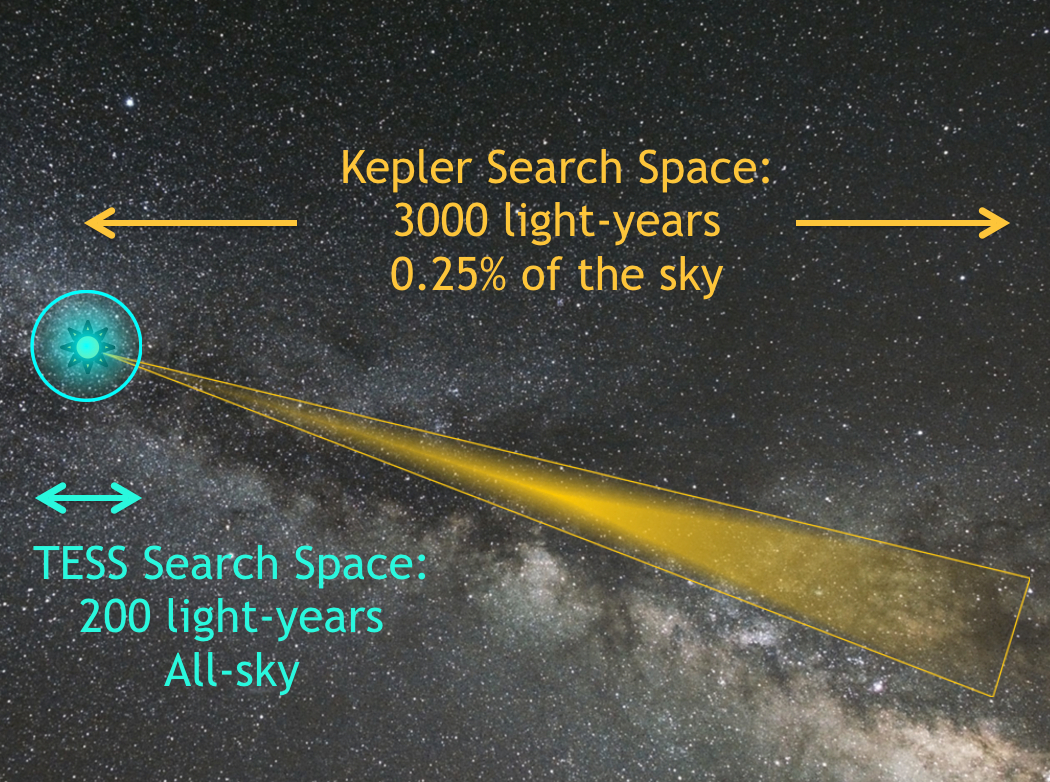
\includegraphics[width=0.9\linewidth]{figures/images/TESS_vs_Kepler}
    \caption{Comparison of the survey strategies of the \textit{Kepler} and TESS missions\protect\footnotemark[4]{}. \textit{Kepler} focused on a deep search of a small region of the sky, while TESS conducts a wide-field survey targeting nearby stars across nearly the entire sky.}
    \label{fig:TESS_vs_Kepler}
\end{figure}

\footnotetext[4]{\url{https://www.nasa.gov/space-science-and-astrobiology-at-ames/division-overview/astrophysics-branch-overview-sta/exoplanet-mission/exoplanet-research-projects}}

Following the success of the \textit{Kepler} and K2 missions, NASA launched the Transiting Exoplanet Survey Satellite (TESS) to carry out a wide-field survey of nearly the entire sky, focusing on nearby, bright stars well suited for follow-up characterization \citep{Ricker2015, Huang2018}. This observing strategy puts emphasis on short-period planets orbiting luminous host stars which are better suited for precision mass measurements and atmospheric studies.

TESS monitors the sky in sectors with typical observing baselines of $\sim27$ days each. Compared to \textit{Kepler}, which maintained continuous observations of the same field, this is significantly shorter. Figure~\ref{fig:TESS_vs_Kepler} shows an artist rendition of the field of view covered by TESS in comparison to that of \textit{Kepler}. As a result, TESS is most sensitive to planets with orbital periods shorter than $\sim10$–$20$ days. Longer period planets remain better constrained by the extended \textit{Kepler} dataset \citep{Sullivan2015}. Despite this limitation, TESS has greatly expanded the known population of transiting exoplanets and produced thousands of candidates orbiting bright nearby stars across the sky \citep{Guerrero2021}.

Together, \textit{Kepler} and TESS complement one another on insights into exoplanet populations. The long baseline and high photometric precision of \textit{Kepler} allowed for statistical studies of population occurrence rates and structure. One prominent result is the discovery of the “radius valley”, a deficit of planets with radii around $1.5$–$2R_{\oplus}$ that separates two dominant populations of super-Earths and sub-Neptunes \citep{2017AJ....154..109F, 2018MNRAS.479.4786V}. In contrast, TESS primarily detects planets orbiting bright nearby stars, making these systems well suited for detailed follow-up observations. These include radial velocity mass measurements and atmospheric characterization with facilities such as the James Webb Space Telescope. TESS is the connection between the statistical studies of exoplanet populations and parameter estimation of planetary systems \citep{Batalha2019}.

\subsection{PLAnetary Transits and Oscillations of stars (PLATO)} \label{sec:PLATO}

Looking ahead, the European Space Agency (ESA) is preparing the next major mission in exoplanet transit research. Known as the \textit{PLAnetary Transits and Oscillations of stars} (PLATO) mission, its objective is to extend the work \textit{Kepler} and TESS by introducing high-precision, long-baseline photometric monitoring of bright stars across large areas of the sky \citep{Rauer2014}. The mission is currently scheduled to launch between late 2026 and early 2027. PLATO's primary goal is to detect and characterize terrestrial exoplanets orbiting within the habitable zones of their host stars. Furthermore, the mission will perform asteroseisomology to determine precise stellar ages, radii, and masses.

PLATO will combine wide-field coverage with long-duration observations lasting several years in selected fields. In contrast to TESS, PLATO's strategy is optimized for detecting small planets with longer orbital periods which are much more difficult to observe with current all-sky transit surveys \citep{Rauer2014}. The mission is expected to produce a statistically robust sample of Earth-sized planets with well constrained host-star properties. Such measurements will enable detailed study of planetary system evolution and improve estimates of habitable worlds in the solar neighbourhood. 

Together, PLATO, \textit{Kepler}, and TESS form a complementary sequence of transit surveys. Collectively, they span deep narrow-field observations, all-sky coverage of bright stars, and future baseline characterization of nearby terrestrial systems.  Within this progression, PLATO is anticipated to provide the precise stellar and planetary parameters necessary to connect statistical exoplanet demographics with detailed physical characterization \citep{PLATO2022}.
\end{comment}